\documentclass[a4paper, 11pt]{article}
\usepackage{comment} % enables the use of multi-line comments (\ifx \fi) 
\usepackage{lipsum} %This package just generates Lorem Ipsum filler text. 
\usepackage{fullpage} % changes the margin
\usepackage{hyperref}
\usepackage{graphicx}

\begin{document}
%Header-Make sure you update this information!!!!
\noindent
\large\textbf{Assignment 1} \hfill \textbf{Tyler Wilding} \\
\normalsize COSC 2596 \hfill Due Date: 20/09/16 \\
Dr. Miguel Garcia-Ruiz \hfill \\
TA: -- \hfill 

\section*{Initial Thoughts}
For my product analysis, I decided to just look at a simple TV, mainly the TV configuration menu that the remote is used to interact with.  The TV I looked at is not terribly old, only around 3-5 years old, and I overall enjoy using it when I need to.  The number one thing that I like about these older TVs is that the software was still designed in a simple manner, it may not look the best but it is functional.  What I mean by this is that the menus are not flashy and animated, all actions with the TV have instant feedback which for me is one of the most important features when working with a digital device.  I do not want to have to wait long periods of delay just to navigate a menu while using an already chunky remote.  This is something that I do not like about newer TVs, in the effort to make the configuration menus simpler and well layed out, it does the opposite for me.  I spend much more time navigating menus and waiting after each button press for the animations to finish only to find that the settings I want to change aren't even available to me.  This is not to say that the older TV is without it's flaws, I feel that some of the options in the menus are confusing, and while I have a good idea of what they are changing, it feels like they could have displayed more effectively.  I don't understand why TV remotes always have to be cluttered with so many buttons when the vast majority of users only use a very small selection of buttons and that is another thing that this TV does well.  Other than that however, I can't really complain about anything in the simple TV menu, it is one of the better one I've seen.  Below are pictures of the TV I used and it's respective remote, as well as pictures of a newer TV that I drew some of my comparisons from.\\

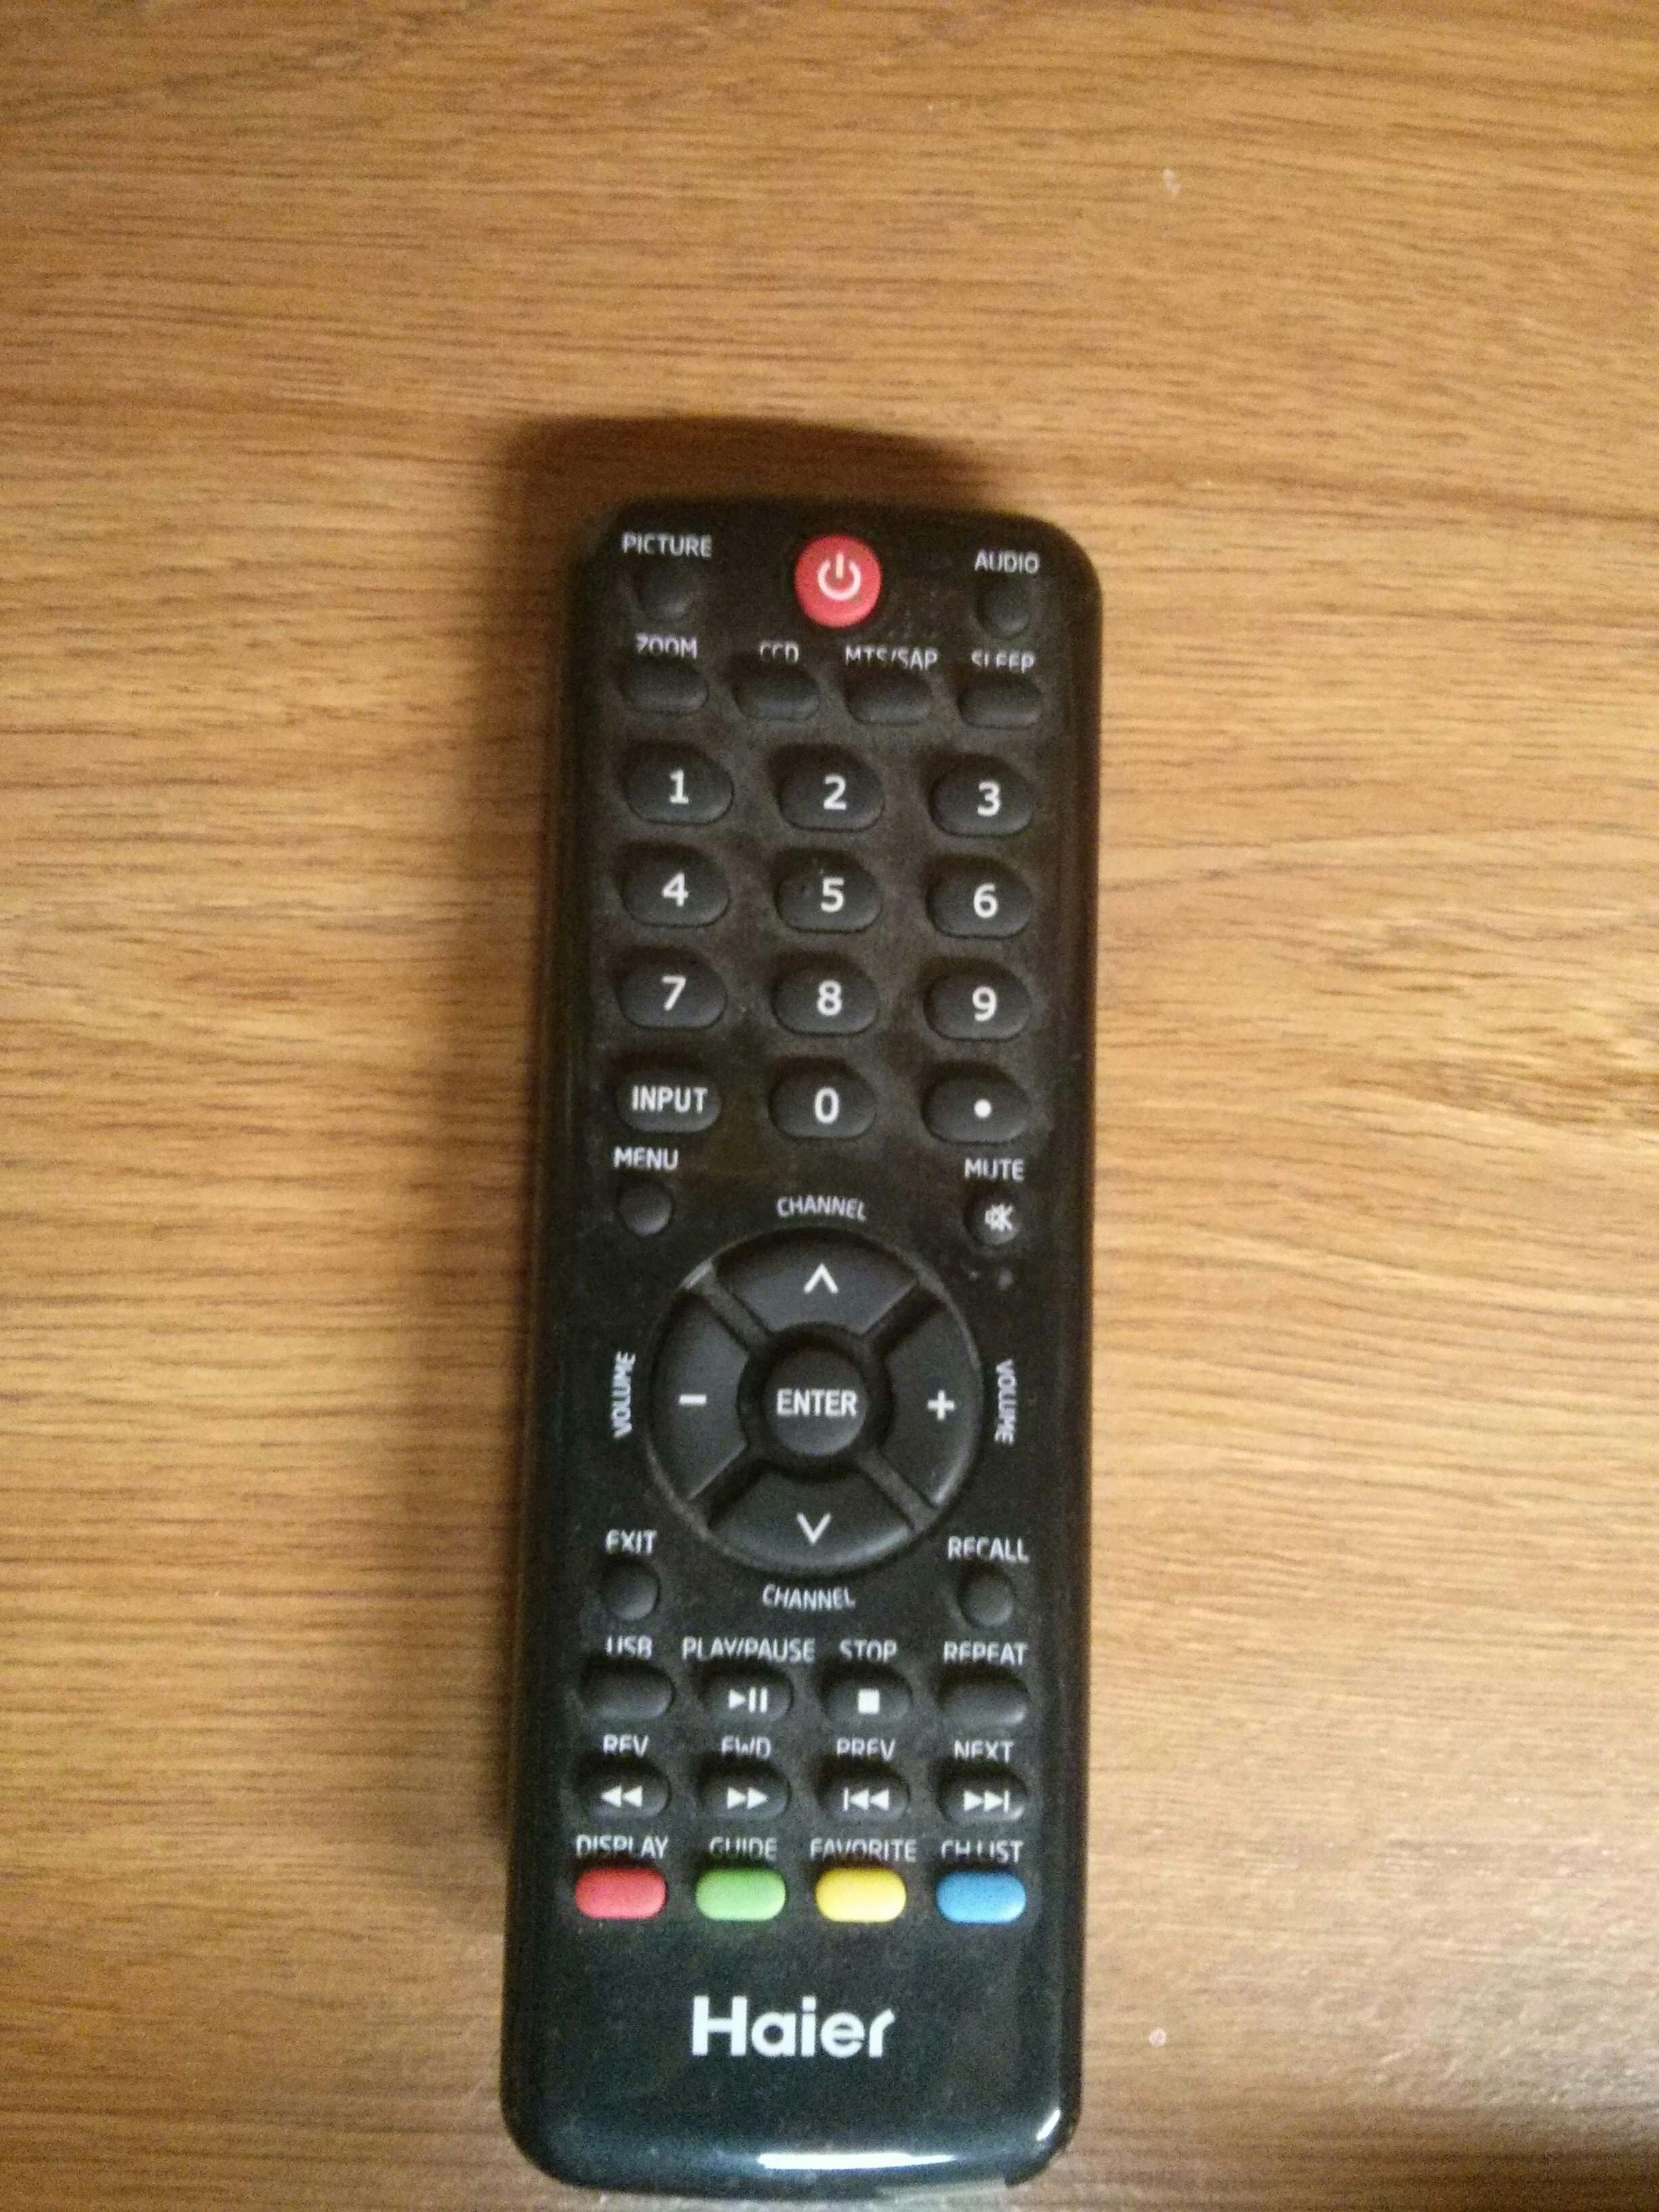
\includegraphics[width=200px,height=200px]{remoteold.jpg}
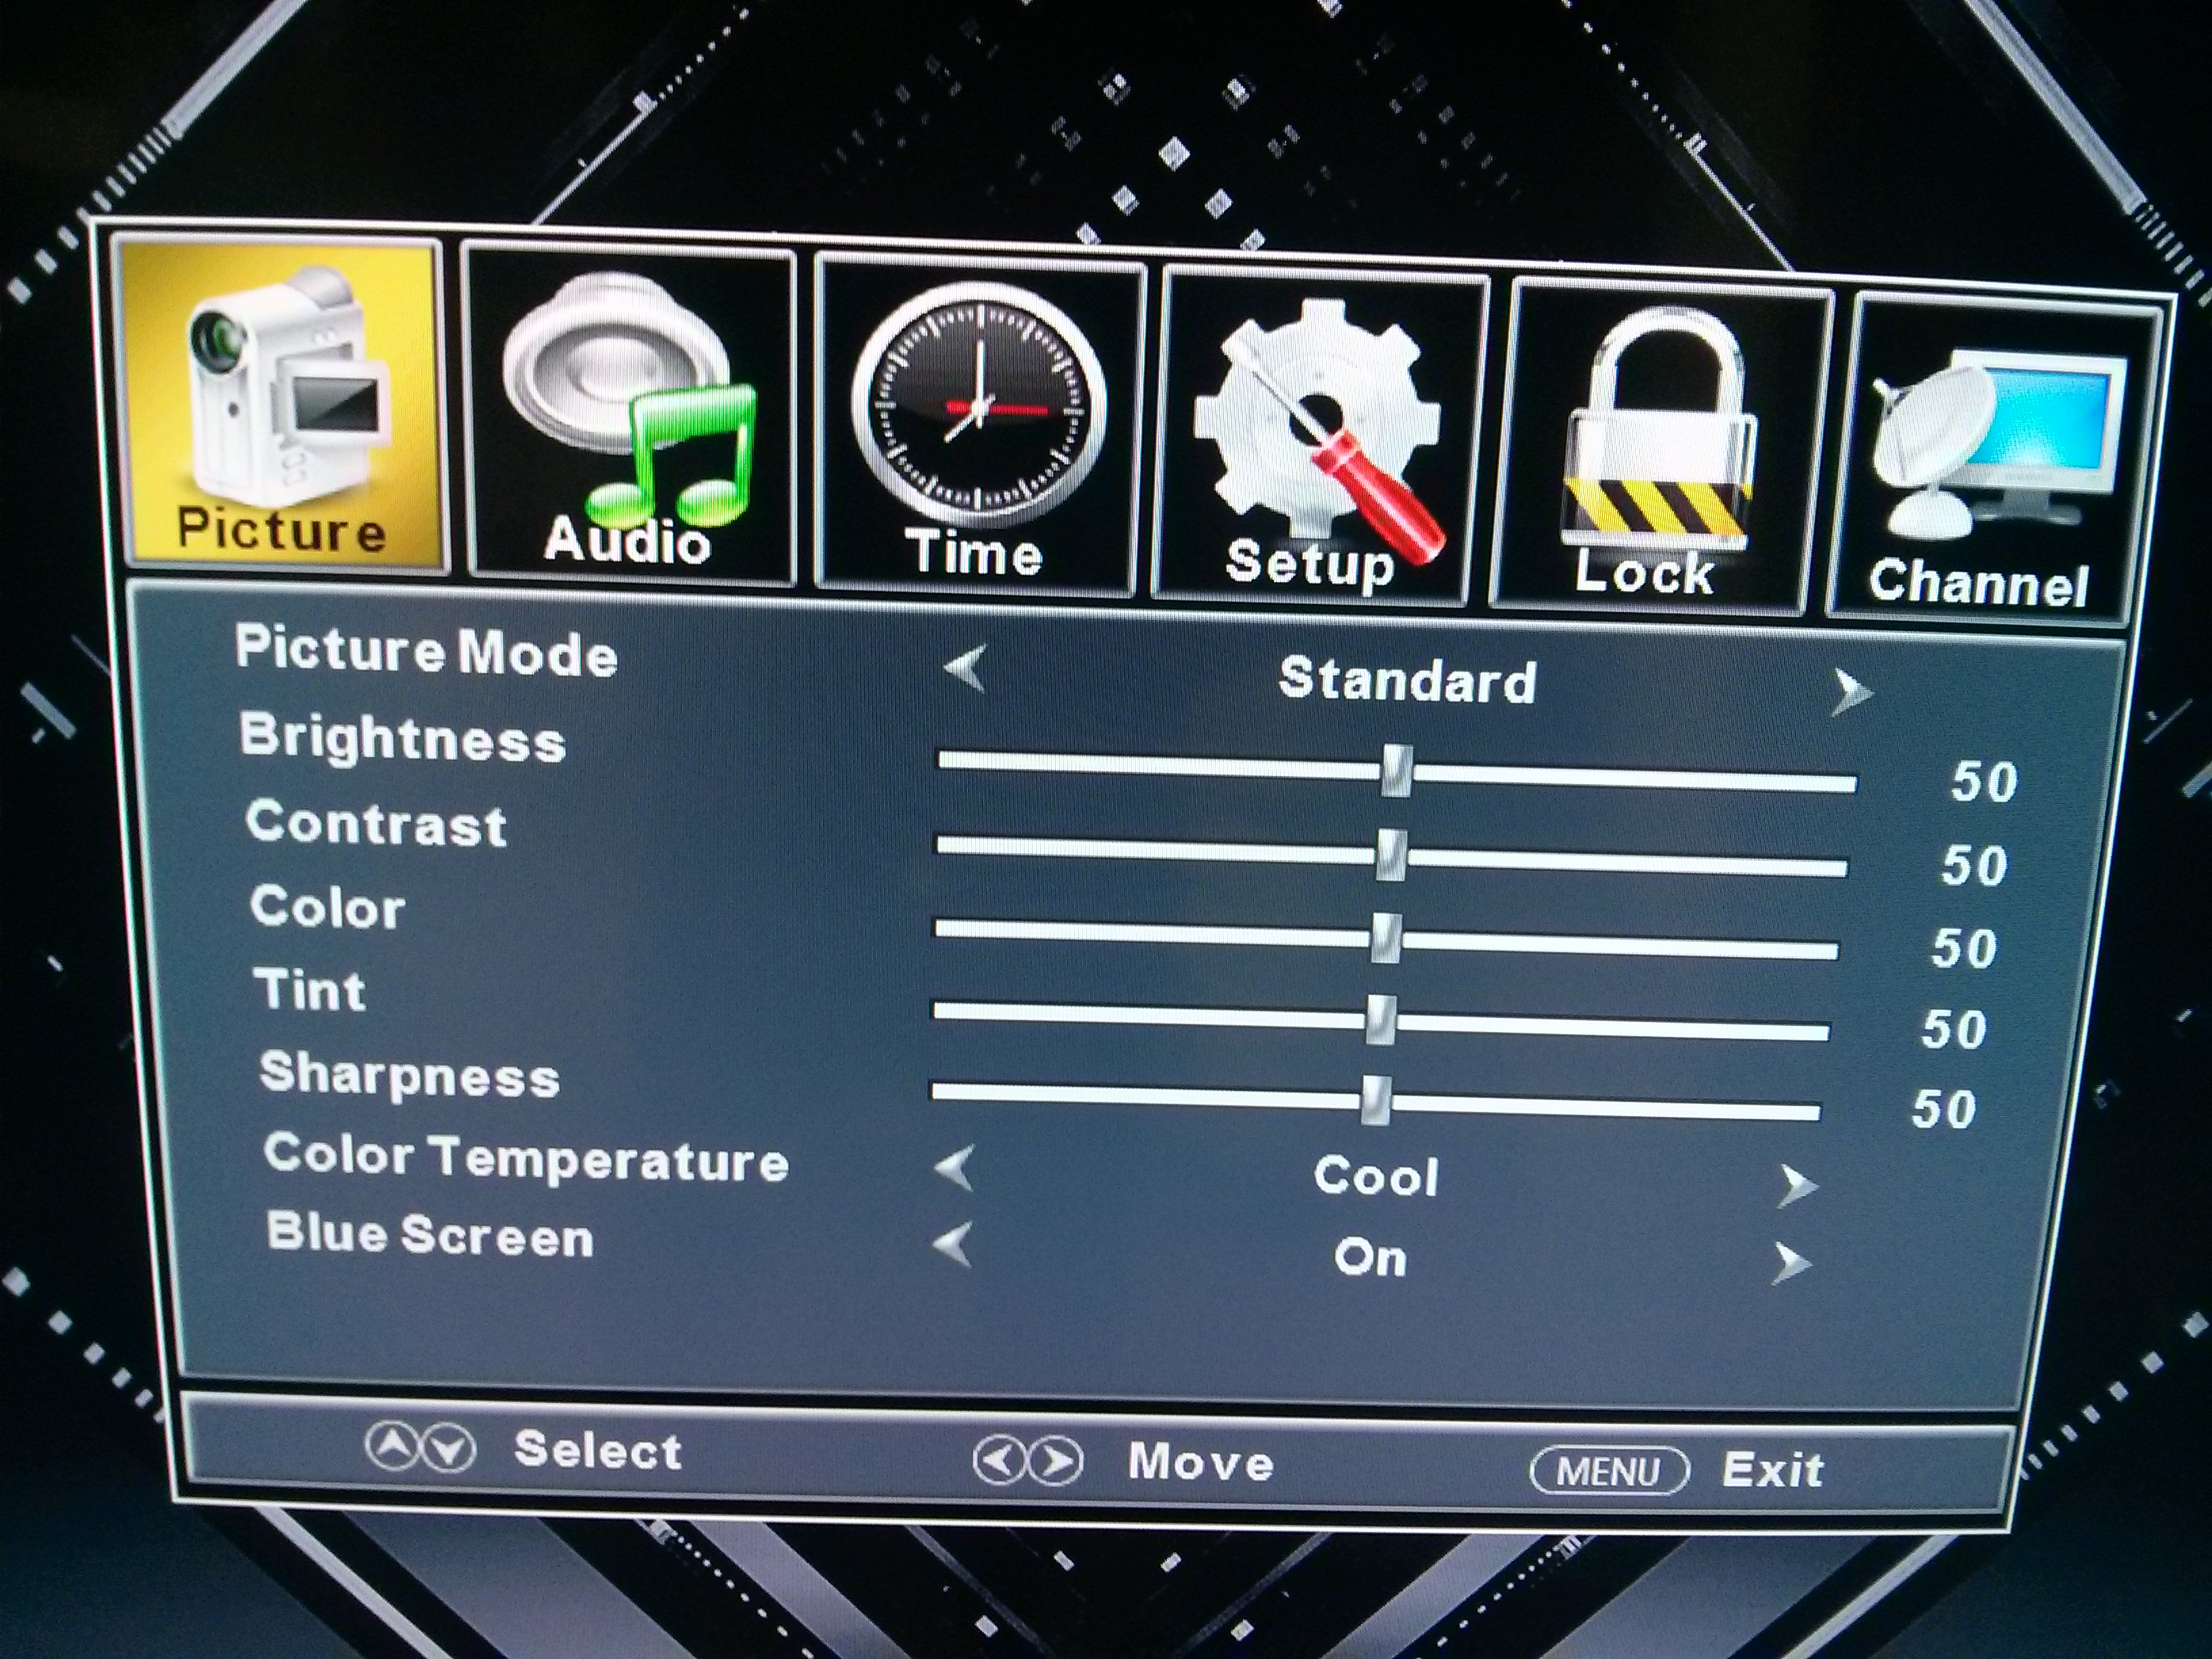
\includegraphics[width=200px,height=200px]{menuold.jpg}\\

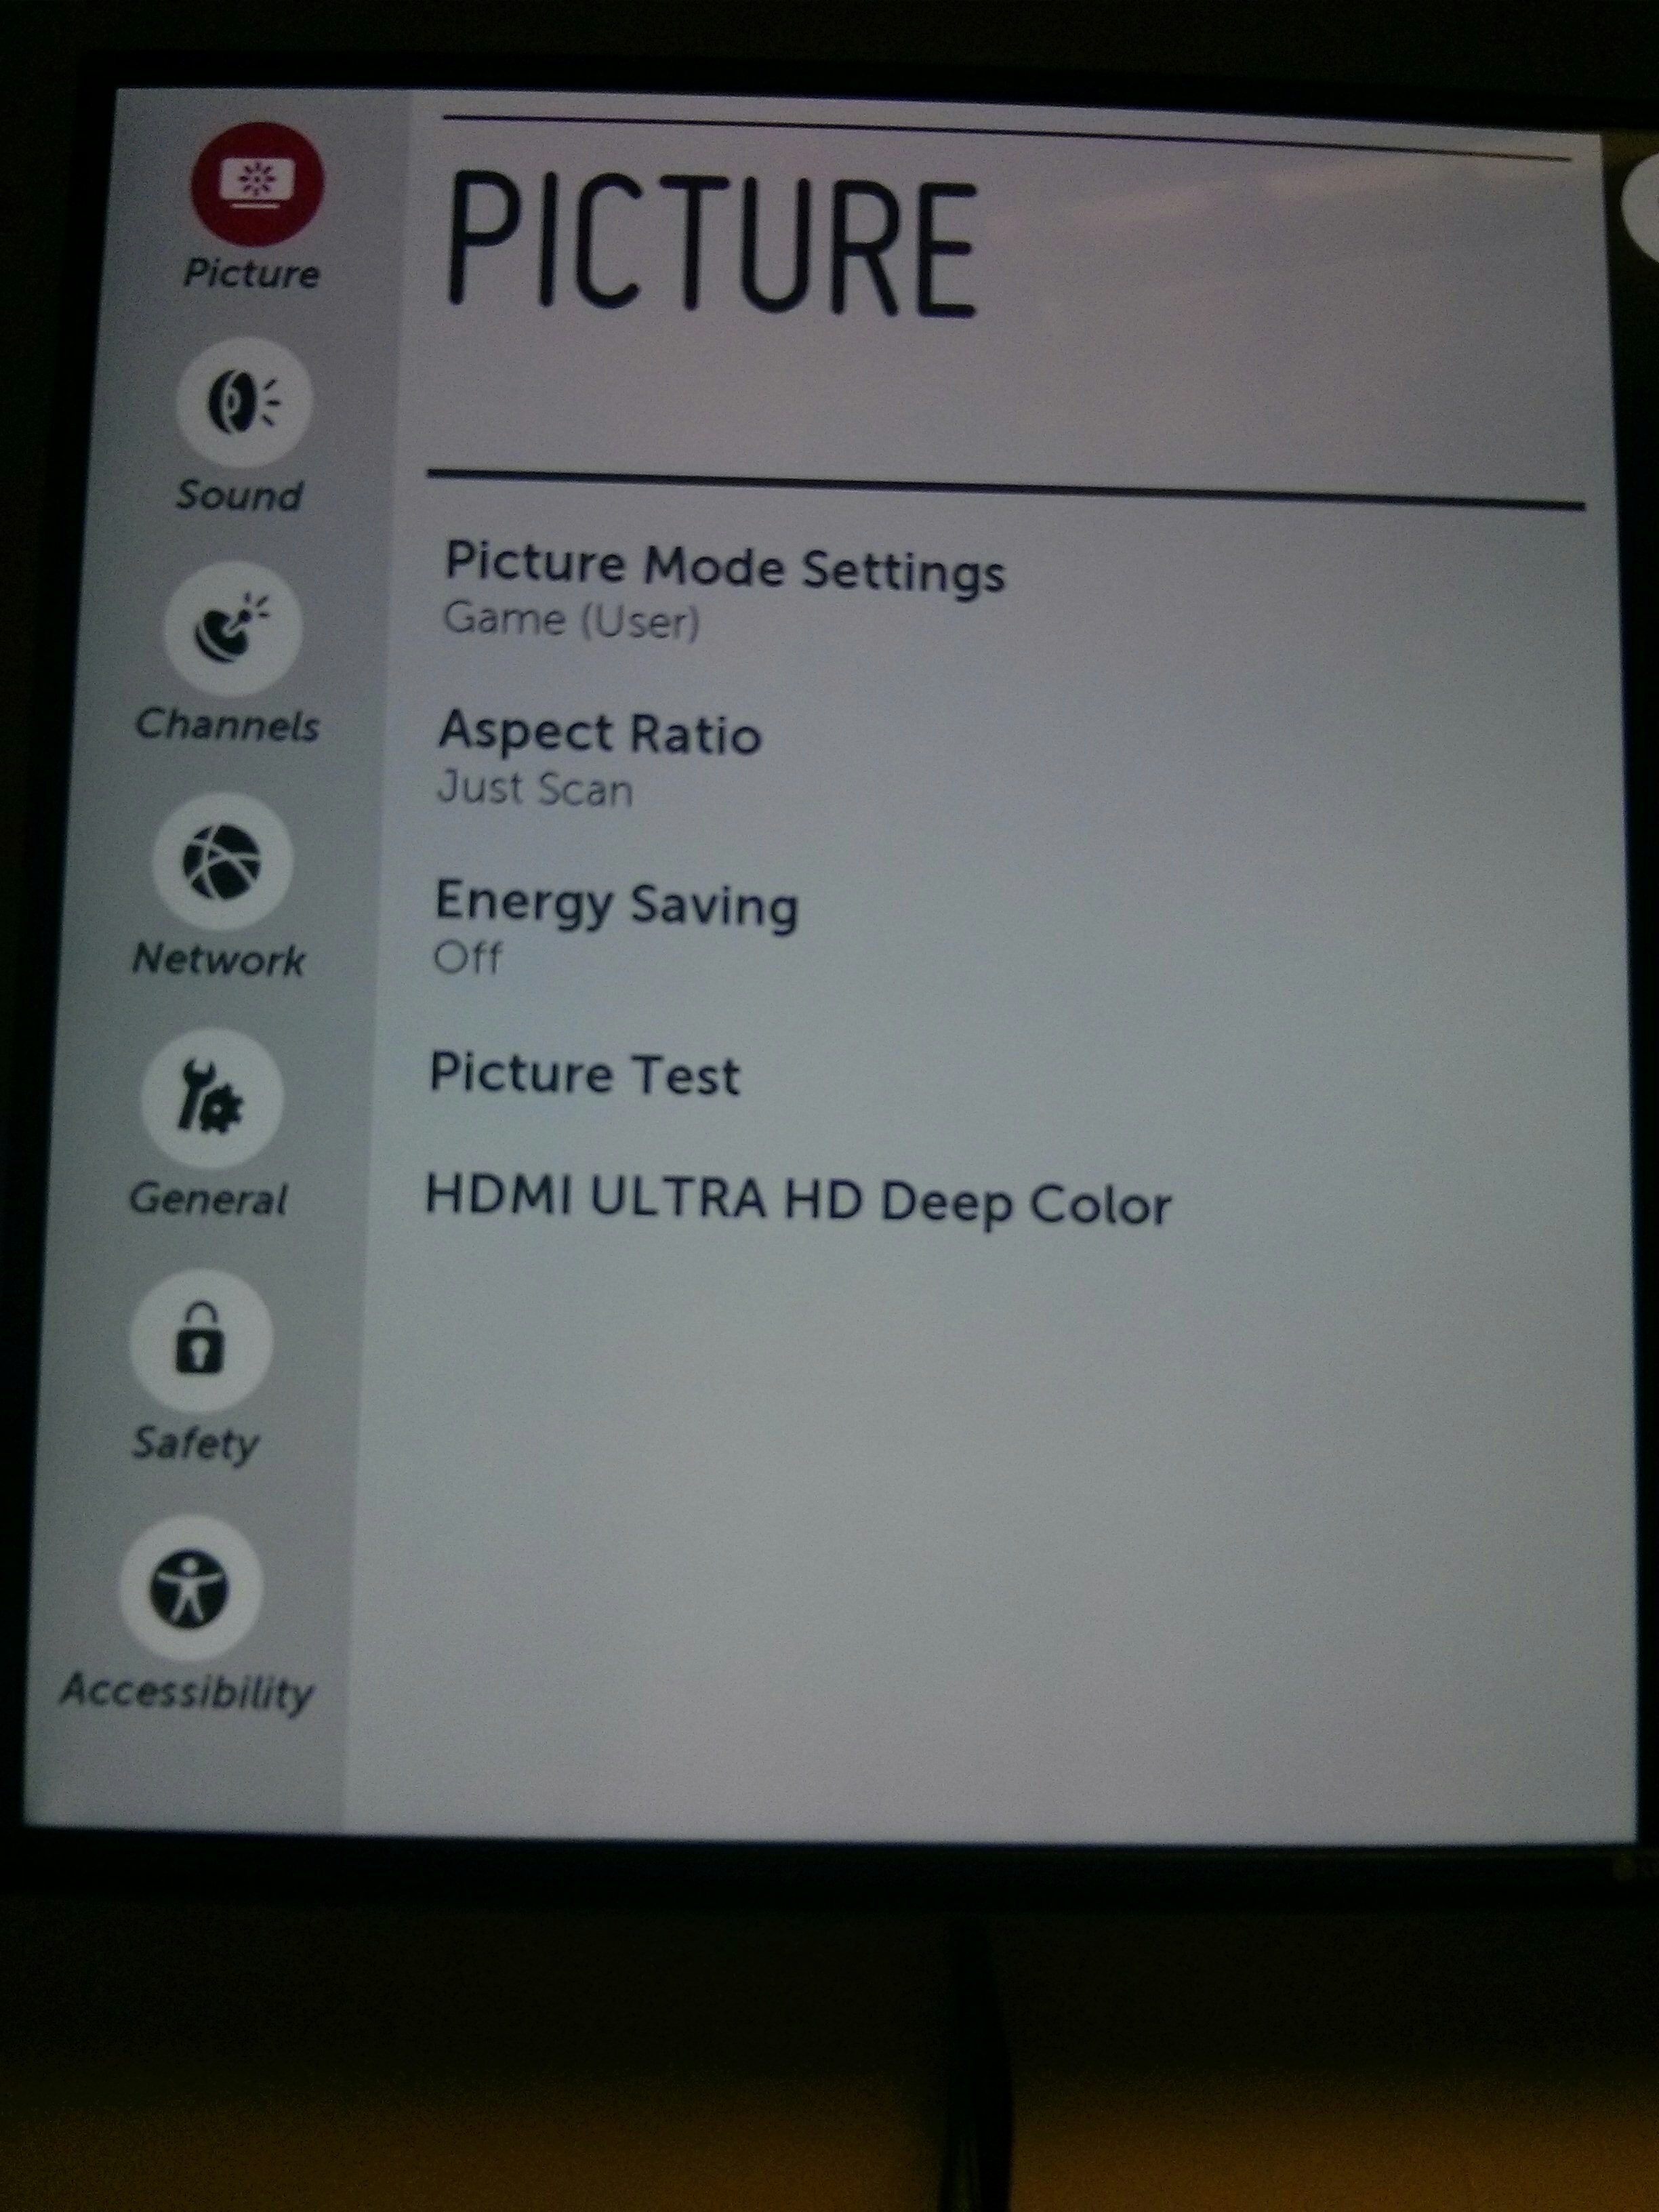
\includegraphics[width=200px,height=200px]{menunew.jpg}
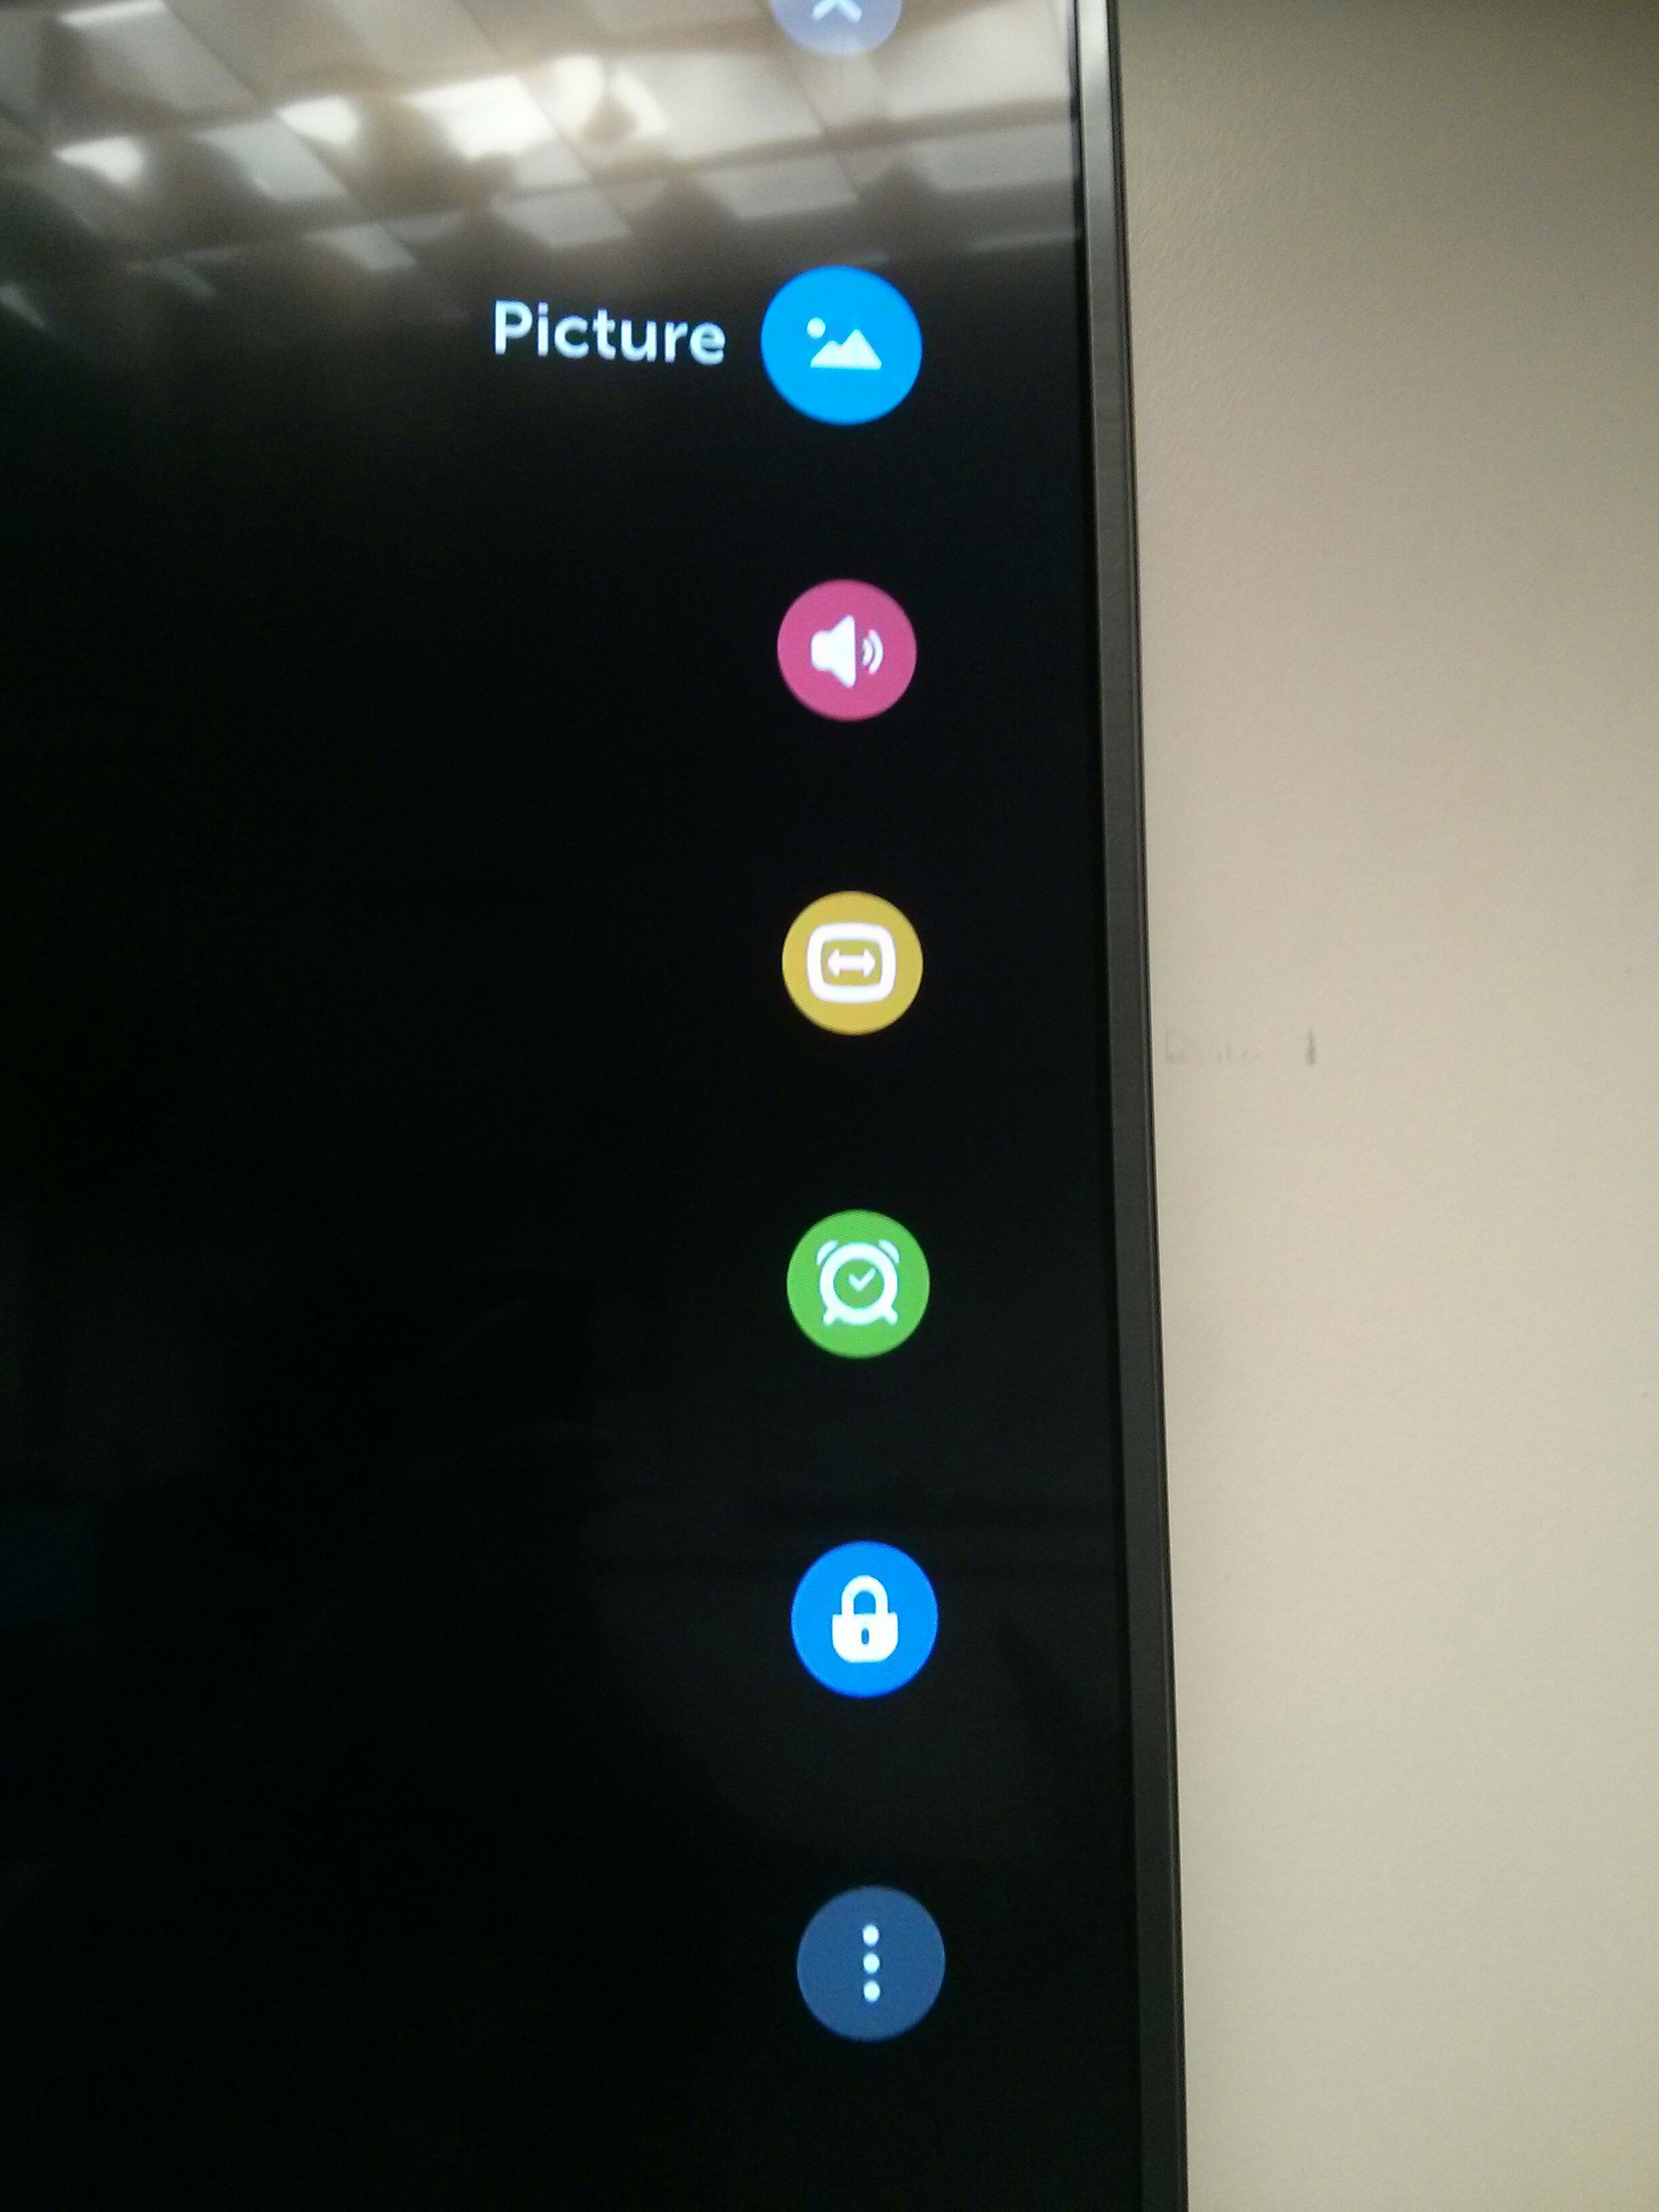
\includegraphics[width=200px,height=200px]{inputnew.jpg}

\section*{Design Principles}

\subsection*{Visibility}
In terms of the menus within the TV themselves, I believe that there is a good amount of visibility.  The colors of the menu are nice contrasting colors, nothing is difficult to read with a simple font. However, what I think could be improved is some of the labeling on the remote itself.  Considering how well spaced out the buttons are, some of the buttons such as the menu button have very small almost hiddne fonts which makes it difficult to read.

\subsection*{Feedback}
As I mentioned, a good feedback is one of the most important things in my opinion, as you are using a very clunky interface with the device in the first place, you are forced to cycle through menus and options so the least the device can provide is speed.  And this TV delivers, going through these menus has almost no delay, as well as changing the options is good because the TV background is unaffected allowing you to immediately see the difference after changing settings.

\subsection*{Constraints}
In terms of constraints, it is not really possible to do anything wrong to mess up the TV, most of these settings are easily reversed and have logical upper and lower bounds that you cannot exceed.  About the only other constraint is the fact that on the security menu you have to enter the password for access.

\subsection*{Consistency}
I think that the TV follows what most people would expect if they ever have configured a TV before, the menu even opens up to probably the most accessed option which is the picture settings.

\subsection*{Affordance}
There are many affordances offered in these menus to help you subconsciously know how to navigate and use it.  Not only are there some what simple instructions at the bottom, but it is clear what each sub-menu does from both the text and the picture along with it.  Similarly, once inside the sub-menu it is easy to tell what options are from a pre-determined list and which are sliders that change a numeric value.

\section*{User Experience and Usability Goals}
In terms of usability goals, I believe that this TV menu achieves it.  The results of changing values and pressing buttons on the remote are effective and efficient with fast response times.  Once you learn where the buttons are on the remote, which are uncluttered it is very easy to learn and use, and if you forget there are enough on-screen clues to guide you in the correct direction.  Compared to the newer TV that has massive latency between actions, has unnessecary complex menu systems that trys to make quick changes faster but ends up taking more time it is much more usable.

In terms of user experience goals, when I use the older TV I feel much more relaxed, confident, and don't feel as if my entertainment or desires are being hindered upon.  On the other hand, with the newer TV because of it's flaws, I often end up feeling bored, unmotivated and frustrated.

\section*{Corrections or Improvements}
One thing that I think could be fixed on the older TV is the security menu.  It only has a single option whe not logged in which just says to enter your password.  This is the one major flaw that I see with this because for one thing, I don't even know the default password I would have to look it up, so I think the default password should be provided.  Also I think that it could elaborate on why you are entering the password, something like, please enter your password to change security settings.  This is the only change I can think of making, 

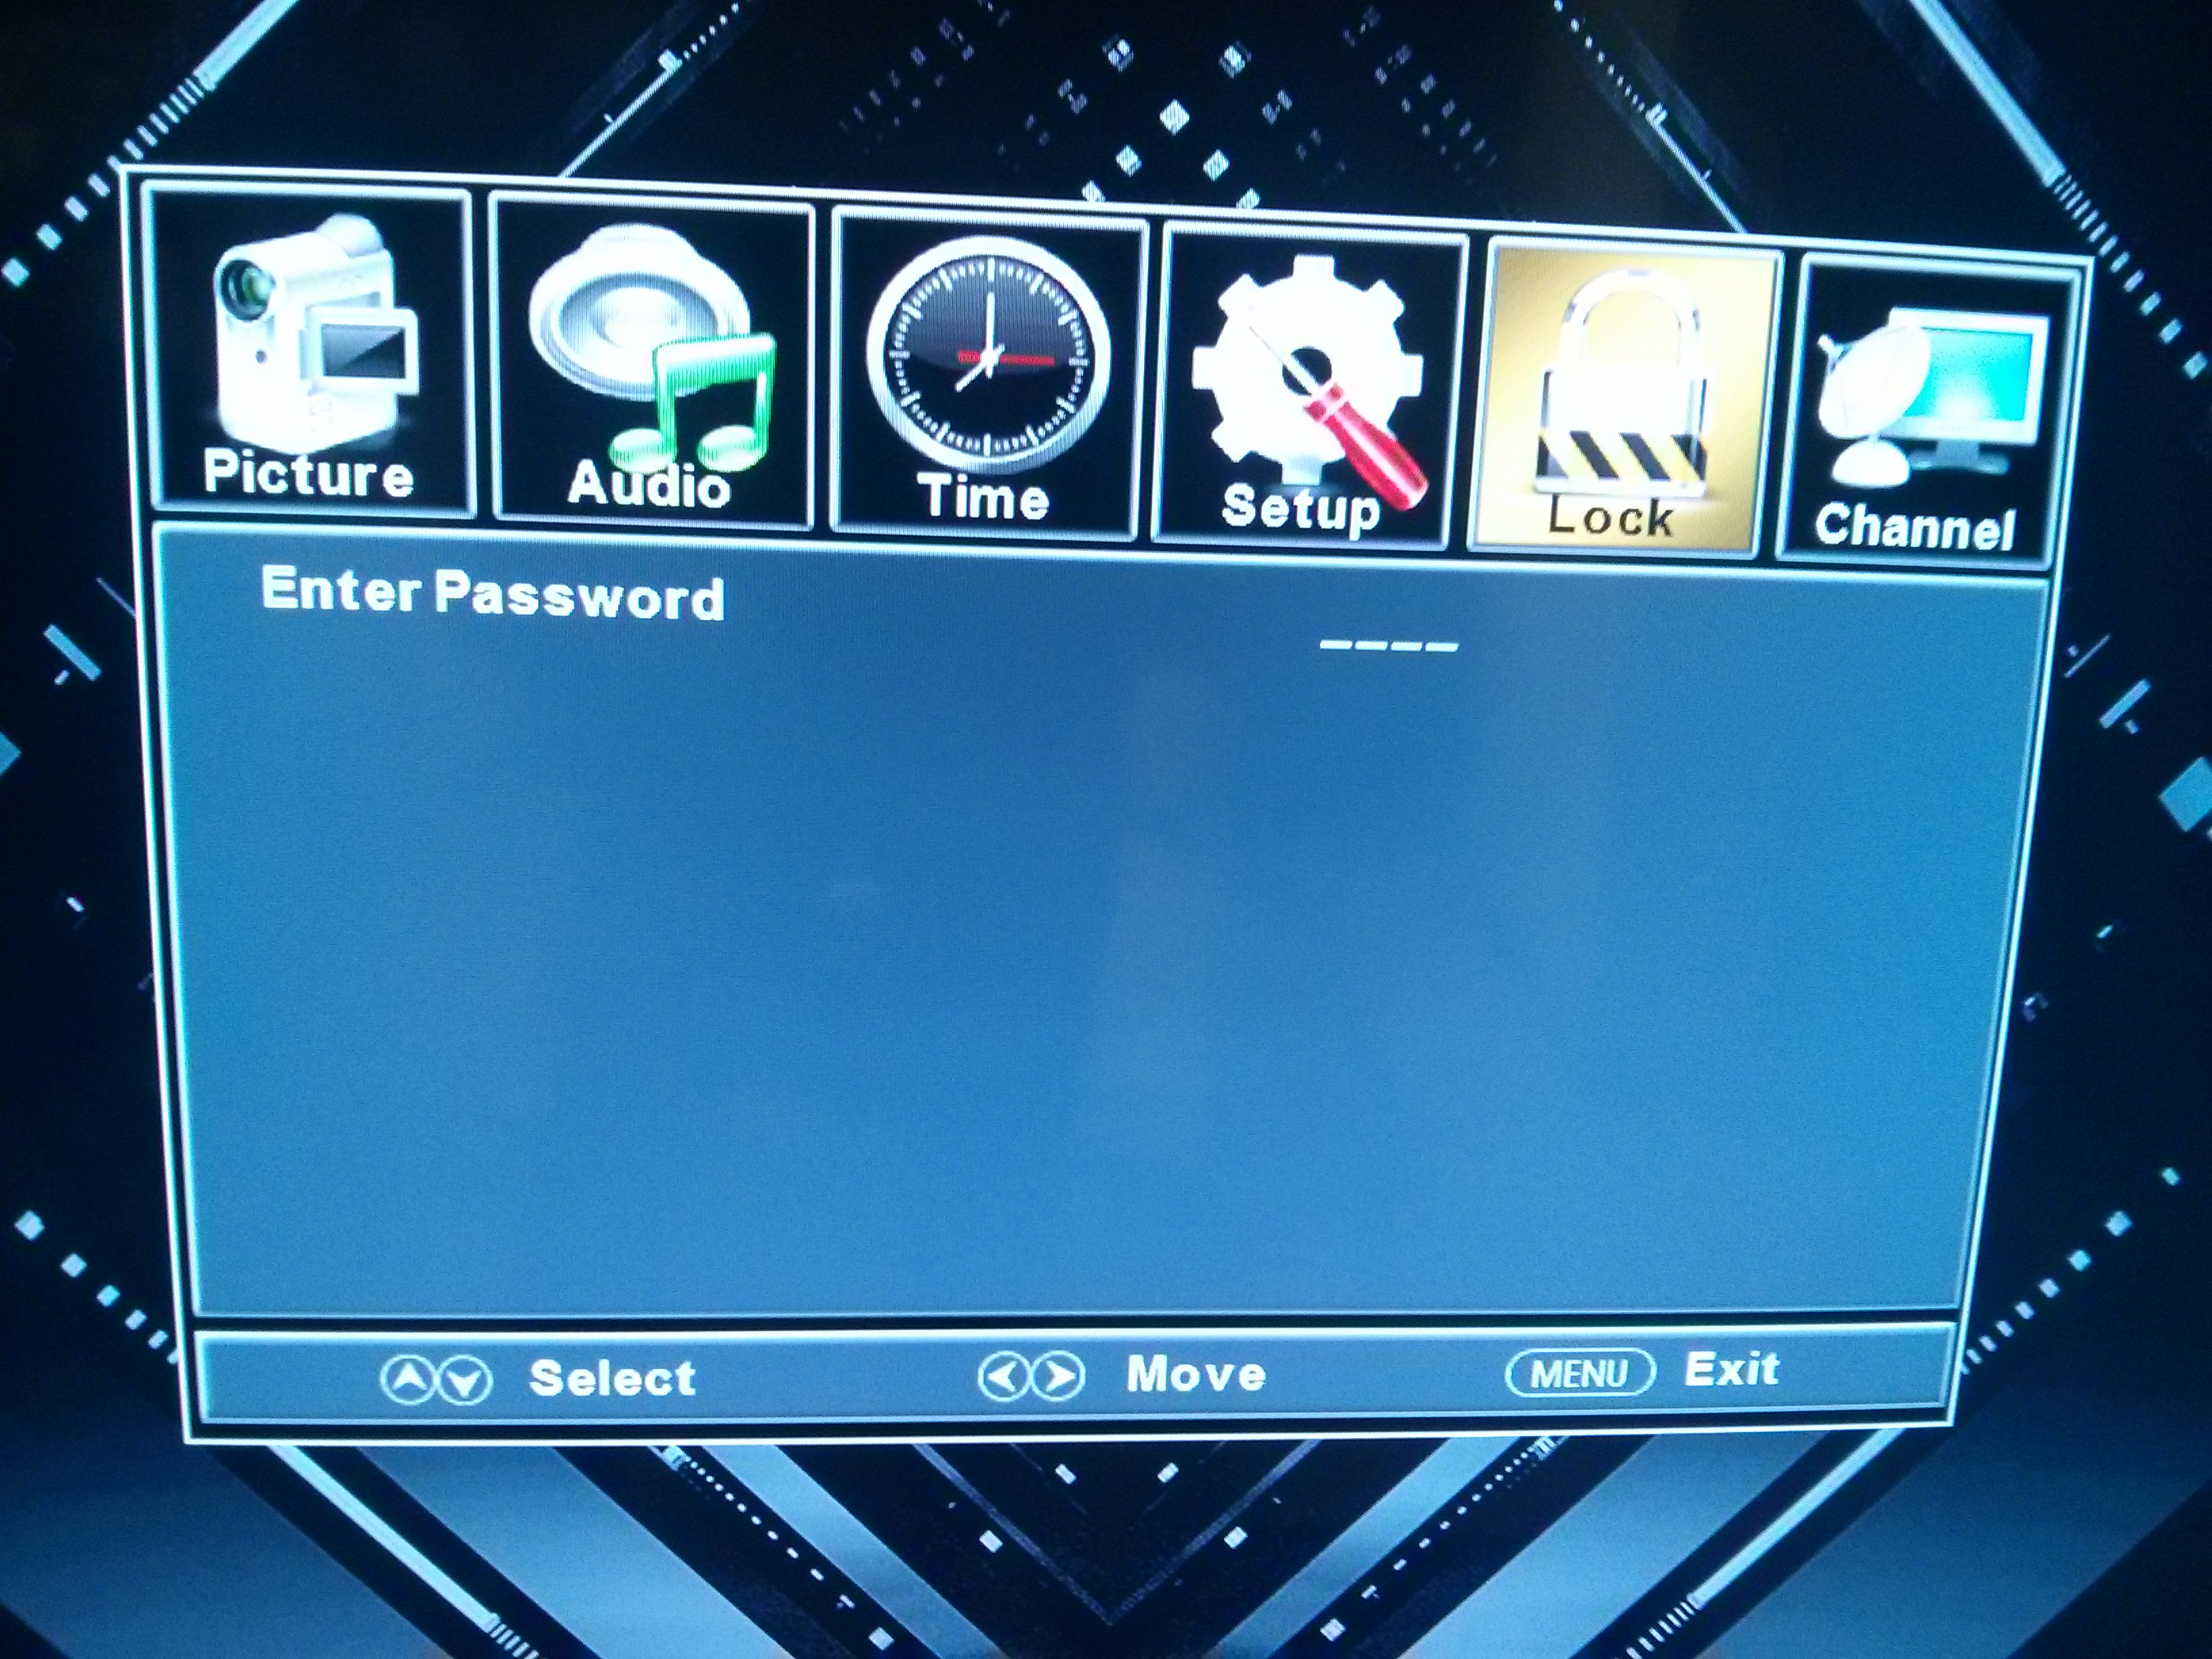
\includegraphics[width=200px,height=200px]{complaintold.jpg}

I think that the menu while simple is very usable and functional and I would not change anything else so I don't think it constitutes making a sketch.  However, I will make a quick sketch on how I think the newer TV menu could be changed to be much more improved.  Also, while I do not have pictures of the newer TV's remote, while the button's text is clearly visible it is very crammed together with not a lot of space inbetween the buttons, another problem with the usability.

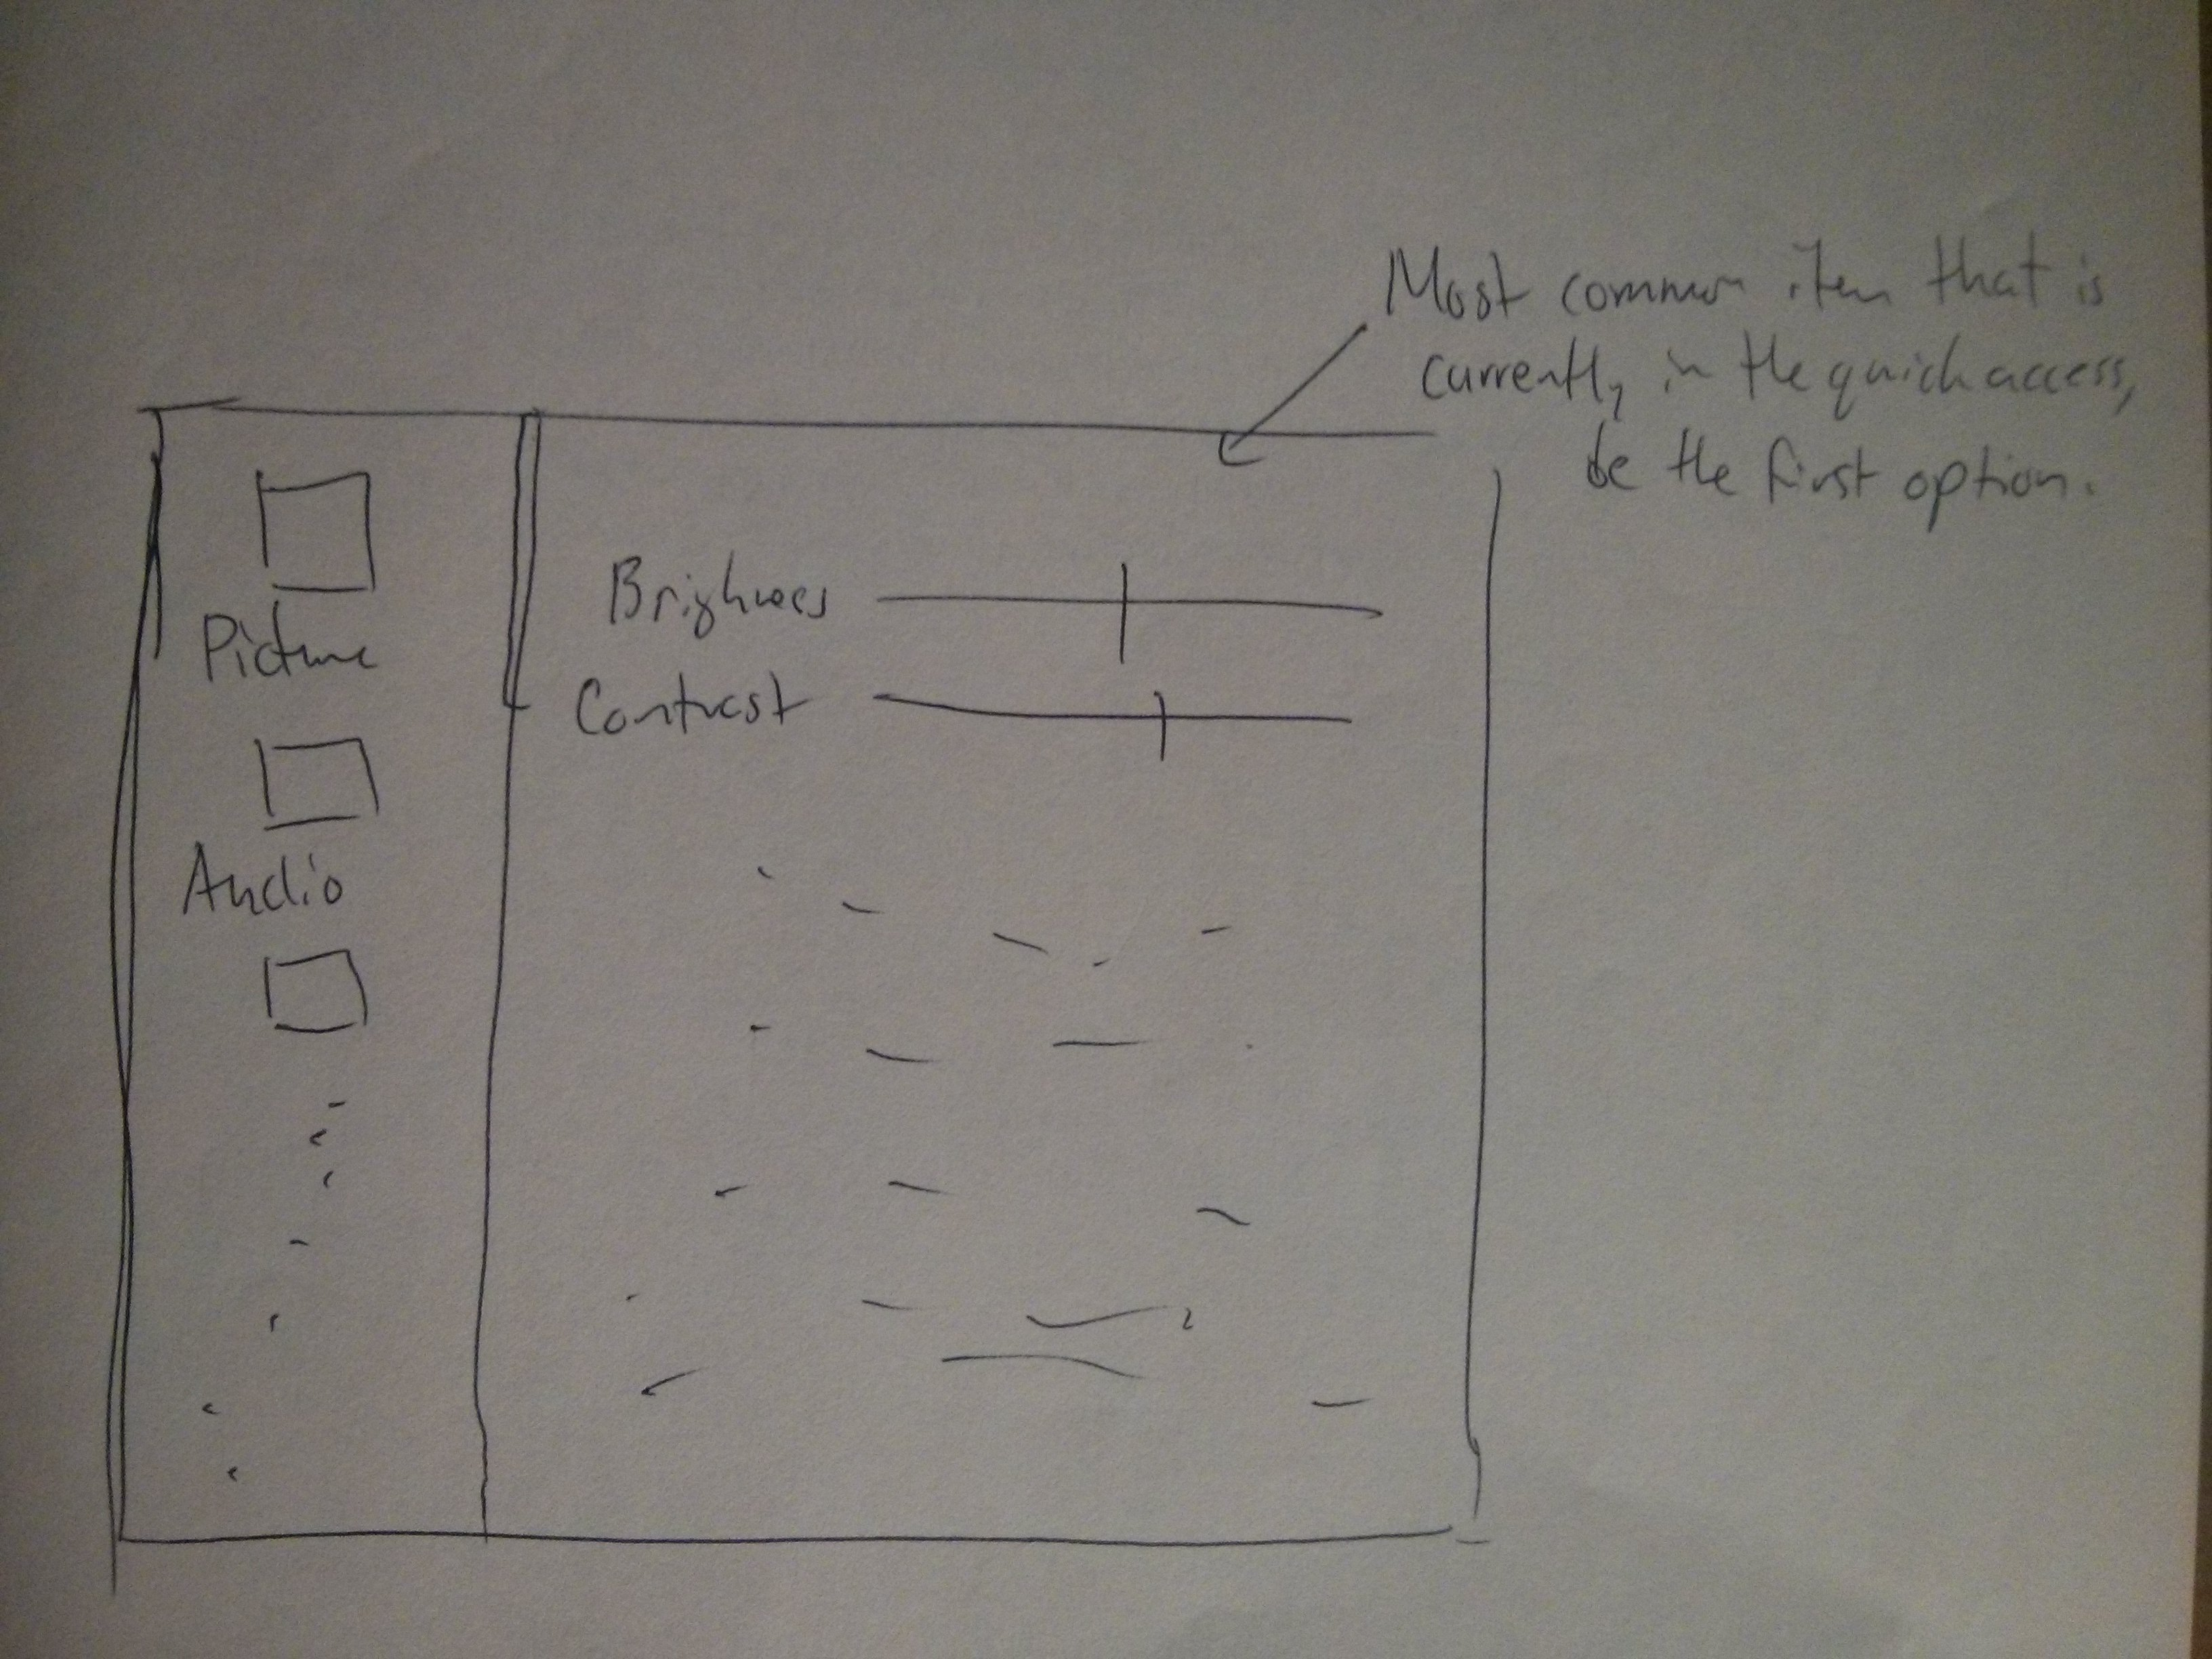
\includegraphics[width=200px,height=200px]{sketch.jpg} \\

In this simple sketch, it tries to take the ideas in their original menu and make it similar to what I liked about the older menu.  The menu button on the remote would immediately open up the dialog that contains all options, with the main categories on the left side.  In each category, the first option would be the option that is available in the quick access menu (before pressing the advanced button at the very bottom).  This keeps all of the functionality, without causing anymore user inputs, however they also have the other options available to them if they need them.  Also, these menus would not have a large delay, sacrificing nice animations for usability.

\section*{Final Word}
In the end, I feel that having a response, fast to use system is much better than trying to create a more modern sleek interface.  I feel that both however can come together effectively, but in the pursuit of one clearly the other one falls short often.  I feel like this is a trend that is occuring in many areas of design at the moment, and why standards that companies like Google puts out like Material design are steps in the right direction.  Through this report I believe I have explored the majority of what there is to analyze for a TV's software and hardware side.

\end{document}
